\documentclass[conference]{IEEEtran}
\IEEEoverridecommandlockouts
\usepackage{cite}
\usepackage{amsmath,amssymb,amsfonts}
\usepackage{algorithm}
\usepackage{algorithmic}
\usepackage{graphicx}
\usepackage{textcomp}
\usepackage{xcolor}
\usepackage{booktabs}
\usepackage{multirow}
\usepackage{array}
\usepackage{tikz}
\usetikzlibrary{arrows.meta,positioning,fit,calc,shapes.geometric,backgrounds}
\usepackage[hidelinks]{hyperref}
\def\BibTeX{{\rm B\kern-.05em{\sc i\kern-.025em b}\kern-.08em
    T\kern-.1667em\lower.7ex\hbox{E}\kern-.125emX}}

\graphicspath{{figures/}}
\newcommand{\gco}{gCO$_2$}
\newcommand{\pp}{\,pp}
\renewcommand{\algorithmicrequire}{\textbf{Input:}}
\renewcommand{\algorithmicensure}{\textbf{Output:}}
\tikzset{
  blk/.style={draw,rounded corners=2pt,align=center,font=\scriptsize,inner sep=3pt,minimum height=0.6cm},
  arr/.style={-{Stealth[length=1.8mm]},semithick},
}

% ------------------------------------------------------------------ edit if needed
\newcommand{\affil}{\textit{Dept. of [Department], [Institution]}\\Coimbatore, India}
% ----------------------------------------------------------------------------------

\begin{document}

\title{PACE: Carbon- and SLA-Aware Edge--Cloud Task Scheduling with Preference-Conditioned Deep Reinforcement Learning}

\author{\IEEEauthorblockN{Nandu Manoj}
\IEEEauthorblockA{\affil \\ CB.SC.U4AIE23321}
\and
\IEEEauthorblockN{Naren Sundar L}
\IEEEauthorblockA{\affil \\ CB.SC.U4AIE23322}
\and
\IEEEauthorblockN{Vatturu Pardheev}
\IEEEauthorblockA{\affil \\ CB.SC.U4AIE23344}
\and
\IEEEauthorblockN{Charuvarthan T}
\IEEEauthorblockA{\affil \\ CB.SC.U4AIE23359}
}

\maketitle

% ==================================================================== abstract
\begin{abstract}
Edge--cloud platforms must decide for every task of every job whether to run it on an edge device, a nearby fog server or a distant cloud region. In India the nearby compute runs on a carbon-intensive grid, while clean grids are hundreds of milliseconds away, so neither running locally nor running green is right for every job. The base paper, MERSEM, plans whole jobs once per fifteen-minute epoch with an evolutionary search and a fixed weight between service-level violations and carbon. We present PACE, a deep reinforcement learning scheduler that places each ready task online in about one millisecond. A single preference-conditioned policy, trained with behaviour cloning and proximal policy optimization on domain-randomised simulations, covers the whole trade-off through an input weight; a proportional-integral controller adjusts that weight at run time to hold an operator's service-level target, and a safety shield removes placements that would clearly miss a deadline. In simulation on the base paper's dataset, PACE misses 1.3 percent of deadlines against 13.3 percent for MERSEM with 22 percent less dynamic carbon, keeps its lead under load, failures and estimate errors, and generalises to three of four unseen setups. On a real testbed with laptop edge workers in Coimbatore and cloud instances in Mumbai and Stockholm, PACE missed fewer deadlines than MERSEM in all six paired runs and matched the strongest heuristic with 15 percent less carbon. We also report three sim-to-real gaps the testbed exposed and how we closed them.
\end{abstract}

\begin{IEEEkeywords}
edge computing, cloud computing, carbon-aware scheduling, deep reinforcement learning, proximal policy optimization, DAG scheduling, service level agreement, sim-to-real
\end{IEEEkeywords}

% ==================================================================== I
\section{Introduction}
A smart-city platform runs three kinds of work on shared infrastructure: \emph{safety alerts} from junction cameras that must be detected within about one second, \emph{graph analytics} over the road network that need seconds, and \emph{batch analytics} that may finish within hours. The compute spans three tiers. In our setting the edge is in Coimbatore, the fog is AWS Mumbai (about 30\,ms away, on a grid of roughly 650\,\gco/kWh) and the cloud is AWS Stockholm (about 150\,ms away, roughly 35\,\gco/kWh). Every placement trades latency against carbon, and the best choice changes with load, the hour's grid intensity, the network and node failures.

Reinforcement learning (RL) suits this problem: decisions are frequent and repetitive, the best action depends on a joint state that is hard to model by hand (queues, carbon, network, position in the job's directed acyclic graph, DAG), the outcome is delayed until the job ends, and heuristics must be re-tuned whenever the objective changes. Our base paper, MERSEM~\cite{mersem}, defines this problem but plans offline per epoch, places whole jobs on one machine, fixes the SLA--carbon weight, assumes perfect knowledge and is evaluated in simulation only.

\textbf{Contributions.} (i) Online, task-level placement with a size-agnostic policy that scores every candidate node with a shared network. (ii) One preference-conditioned policy for the whole SLA--carbon trade-off, an online SLA-target controller and a safety shield. (iii) Robustness through domain randomisation and a deferral action. (iv) Real-system evidence: the same scheduler code runs in our simulator and on a real AWS + laptop testbed, with paired statistics and a measured sim-to-real gap. Each ingredient has precedents (Section~\ref{sec:related}); the contribution is their combination for this problem and its validation on real machines.

% ==================================================================== II
\section{Background and Related Work}\label{sec:related}
\subsection{Base paper: MERSEM}
MERSEM~\cite{mersem} schedules graph-analytics DAG jobs on an edge--fog--cloud system. Once per epoch of $\Delta=15$\,min, a predictor supplies the next jobs and a hybrid evolutionary algorithm searches a job-to-machine mapping $x$ that minimises
\begin{equation}
F(x) = w_s\, \mathrm{SLA}(x) + w_c\, \widehat{\mathrm{CO}}_2(x),\qquad w_s+w_c=1, \label{eq:mersem}
\end{equation}
where tabular Q-learning chooses how many jobs a local-search step reassigns (five actions, one step per episode). It is evaluated in an extended EdgeCloudSim~\cite{edgecloudsim} on the Rezaee--Adabi DAG dataset~\cite{dataset}. Table~\ref{tab:critique} lists its assumptions that matter most in practice. Inspecting the dataset we found 51,895 jobs and 1.30\,M tasks, a median of 16 tasks per job, usable job-level deadlines, and empty ``real'' and ``predicted'' runtime columns, so we inject estimate error ourselves.

\begin{table}[t]
\caption{Base-paper assumptions and how PACE addresses them}
\label{tab:critique}
\centering\scriptsize
\begin{tabular}{@{}p{3.85cm}p{4.15cm}@{}}
\toprule
MERSEM & PACE \\
\midrule
Offline plan per 15-min epoch & Online decision per ready task ($\approx$1\,ms) \\
Whole job on one machine, run sequentially & Task-level placement, measured contention \\
Exact runtimes and carbon known & Noisy estimates, randomised in training \\
Fixed weight between a rate and grams & One policy for all $w$; SLA-target controller \\
No failures, priorities or deferral & Masking, re-placement, classes, \textsc{Defer} \\
RL only tunes a perturbation rate & The RL agent is the scheduler \\
Metaheuristic baselines only & EFT, CA-EFT, carbon-greedy, MERSEM \\
Simulation only & Real AWS testbed, measured gap \\
\bottomrule
\end{tabular}
\end{table}

\subsection{Related work}
DeepRM~\cite{deeprm} introduced online RL scheduling in a single cluster, and a follow-up added a behaviour-cloning warm start~\cite{deeprm2}; we reuse both ideas. Decima~\cite{decima} scores DAG stages with a shared network, which inspires our size-agnostic node scorer. Wang et al.~\cite{wang2021} offload dependent tasks with deep RL but without carbon. Preference-conditioned multi-objective RL~\cite{abels2019,yang2019} motivates conditioning on $w$; PID Lagrangian methods~\cite{stooke2020,ray2019} motivate the SLA controller; temporal workload shifting~\cite{wiesner2021} motivates deferral. PPO~\cite{ppo} is our learning algorithm.

% ==================================================================== III
\section{System Model and Problem Formulation}\label{sec:model}

\begin{figure*}[t]
\centering
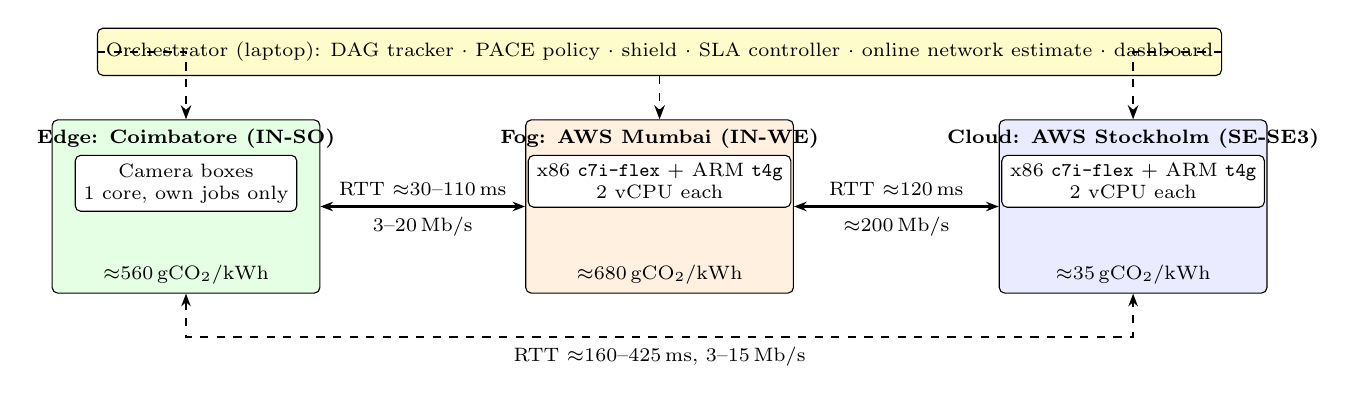
\begin{tikzpicture}[node distance=0.5cm]
% tiers
\node[blk,fill=green!10,minimum width=3.4cm,minimum height=2.2cm] (edge) {};
\node[font=\scriptsize\bfseries,anchor=north] at (edge.north) {Edge: Coimbatore (IN-SO)};
\node[blk,fill=white,below=0.45cm of edge.north] (cam) {Camera boxes\\1 core, own jobs only};
\node[font=\scriptsize,anchor=south] at (edge.south) {$\approx$560\,\gco/kWh};

\node[blk,fill=orange!12,minimum width=3.4cm,minimum height=2.2cm,right=2.6cm of edge] (fog) {};
\node[font=\scriptsize\bfseries,anchor=north] at (fog.north) {Fog: AWS Mumbai (IN-WE)};
\node[blk,fill=white,below=0.45cm of fog.north] (fogn) {x86 \texttt{c7i-flex} + ARM \texttt{t4g}\\2 vCPU each};
\node[font=\scriptsize,anchor=south] at (fog.south) {$\approx$680\,\gco/kWh};

\node[blk,fill=blue!8,minimum width=3.4cm,minimum height=2.2cm,right=2.6cm of fog] (cloud) {};
\node[font=\scriptsize\bfseries,anchor=north] at (cloud.north) {Cloud: AWS Stockholm (SE-SE3)};
\node[blk,fill=white,below=0.45cm of cloud.north] (cloudn) {x86 \texttt{c7i-flex} + ARM \texttt{t4g}\\2 vCPU each};
\node[font=\scriptsize,anchor=south] at (cloud.south) {$\approx$35\,\gco/kWh};

\draw[{Stealth[length=1.6mm]}-{Stealth[length=1.6mm]},thick] (edge.east) -- node[above,font=\scriptsize]{RTT $\approx$30--110\,ms} node[below,font=\scriptsize]{3--20\,Mb/s} (fog.west);
\draw[{Stealth[length=1.6mm]}-{Stealth[length=1.6mm]},thick] (fog.east) -- node[above,font=\scriptsize]{RTT $\approx$120\,ms} node[below,font=\scriptsize]{$\approx$200\,Mb/s} (cloud.west);
\draw[{Stealth[length=1.6mm]}-{Stealth[length=1.6mm]},thick,dashed] (edge.south) -- ++(0,-0.55) -| node[pos=0.25,below,font=\scriptsize]{RTT $\approx$160--425\,ms, 3--15\,Mb/s} (cloud.south);

\node[blk,fill=yellow!20,above=0.55cm of fog] (orch) {Orchestrator (laptop): DAG tracker $\cdot$ PACE policy $\cdot$ shield $\cdot$ SLA controller $\cdot$ online network estimate $\cdot$ dashboard};
\draw[arr,dashed] (orch.west) -| (edge.north);
\draw[arr,dashed] (orch.south) -- (fog.north);
\draw[arr,dashed] (orch.east) -| (cloud.north);
\end{tikzpicture}
\caption{Three-tier system. The edge is close but slow, the fog is near but carbon-heavy, the cloud is clean but far. Grid intensities are annual means; link figures are from our calibration on a campus network.}
\label{fig:system}
\end{figure*}

\subsection{Infrastructure}
The system (Fig.~\ref{fig:system}) has nodes $n\in\mathcal N$, each with $k_n$ execution slots, a speed $s_n$ relative to a reference core, a location $\ell_n$ and a grid zone $z_n$. Locations $a,b$ are joined by links with round-trip time $\mathrm{RTT}_{ab}$ and bandwidth $B_{ab}$.

\subsection{Jobs}
A job $j$ is a DAG $G_j=(V_j,E_j)$ arriving at time $a_j$ from device $o_j$ with deadline $D_j$. Task $i\in V_j$ has work $W_i$ (reference-core seconds), of which the scheduler only sees an estimate $\hat W_i = W_i\,\epsilon_i$, $\ln\epsilon_i\sim\mathcal N(0,\sigma^2)$. Edge $(p,i)\in E_j$ carries $d_{pi}$ megabytes. There are three classes: \textbf{A} safety alerts (deadline 1\,s; 30\% of feeds may not leave India; about 98\% of jobs), \textbf{B} graph analytics (dataset DAGs, $D_j=a_j+2\rho_j\,\mathrm{CP}_j+2$\,s with the dataset's slack ratio $\rho_j$ and critical path $\mathrm{CP}_j$) and \textbf{C} batch (deadlines of 30--120\,min, deferrable). Jobs from the first 70\% of the dataset timeline train and the last 30\% test.

\subsection{Execution, transfer and finish time}
Task $i$ on node $n$ needs the outputs of its parents $P(i)$. A transfer from location $a$ to $b$ takes
\begin{equation}
\tau_{ab}(d) = \tfrac12\mathrm{RTT}_{ab} + \frac{8d}{B_{ab}}, \label{eq:transfer}
\end{equation}
and execution with $u$ of the $k_n$ slots busy takes
\begin{equation}
T^{\mathrm{exec}}_{in} = \frac{W_i}{s_n}\left(1 + c_n\frac{u-1}{k_n-1}\right), \label{eq:exec}
\end{equation}
where $c_n$ is the node's measured contention slowdown (1.7--1.8 for a 2-vCPU x86 instance, about 0 for ARM). Schedulers estimate the finish time as
\begin{equation}
\hat f_{in} = t + \max\!\big(\hat T^{\mathrm{in}}_{in},\, \hat T^{\mathrm{wait}}_{n}\big) + \frac{\hat W_i}{s_n}, \label{eq:finish}
\end{equation}
because input transfers overlap with waiting for a free slot.

\subsection{Energy and carbon}
Following the Cloud Carbon Footprint method~\cite{ccf}, node power interpolates between idle and maximum per-vCPU watts ($P^{\mathrm{idle}}$, $P^{\mathrm{max}}$: 0.74/3.5\,W for x86, 0.47/1.69\,W for ARM) with power usage effectiveness $\mathrm{PUE}=1.135$ in the cloud. The dynamic (scheduler-controllable) carbon of task $i$ on node $n$ is
\begin{equation}
C_{in} = \mathrm{PUE}_n\,\big(P^{\mathrm{max}}_n - P^{\mathrm{idle}}_n\big)\, \frac{T^{\mathrm{exec}}_{in}}{3600}\cdot \frac{I_{z_n}(t)}{1000}\ \ [\mathrm{g}], \label{eq:carbon}
\end{equation}
with $I_z(t)$ the hourly grid carbon intensity (\gco/kWh) of zone $z$, i.e.\ location-based accounting. We report idle carbon separately.

\subsection{Objective}
The service-level violation rate over the class A and B jobs $\mathcal J_{AB}$ is
\begin{equation}
\mathrm{SLA} = \frac{1}{|\mathcal J_{AB}|}\sum_{j\in\mathcal J_{AB}} \mathbb 1\!\left[f_j > D_j\right], \label{eq:sla}
\end{equation}
where $f_j$ is the time the result reaches device $o_j$. The operator wants to minimise $\sum_{i}C_{i,\pi(i)}$ subject to $\mathrm{SLA}\le\varepsilon$, privacy and memory constraints, which we treat with a preference weight $w$ (Section~\ref{sec:method}) and a controller on $w$ (Section~\ref{sec:ctrl}).

% ==================================================================== IV
\section{PACE Methodology}\label{sec:method}

\begin{figure*}[t]
\centering
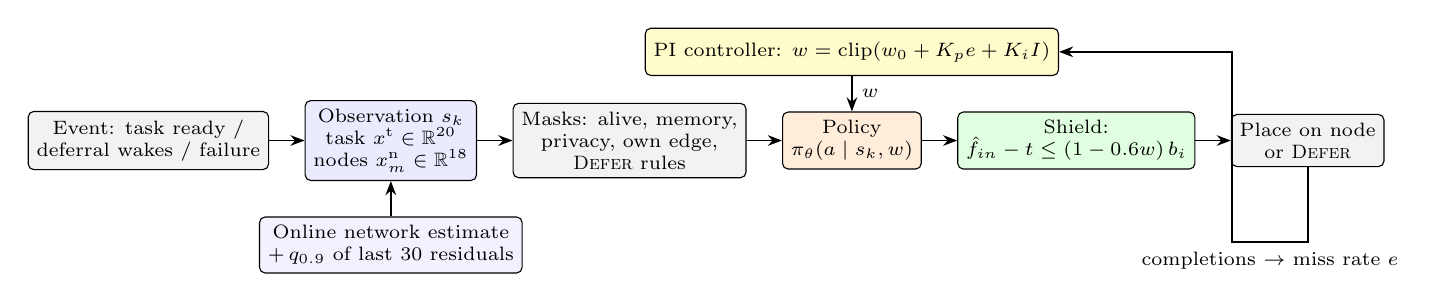
\begin{tikzpicture}[node distance=0.45cm]
\node[blk,fill=gray!10] (ev) {Event: task ready /\\deferral wakes / failure};
\node[blk,fill=blue!8,right=of ev] (obs) {Observation $s_k$\\task $x^{\mathrm t}\in\mathbb R^{20}$\\nodes $x^{\mathrm n}_m\in\mathbb R^{18}$};
\node[blk,fill=gray!10,right=of obs] (mask) {Masks: alive, memory,\\privacy, own edge,\\\textsc{Defer} rules};
\node[blk,fill=orange!15,right=of mask] (pol) {Policy\\$\pi_\theta(a\mid s_k,w)$};
\node[blk,fill=green!12,right=of pol] (sh) {Shield:\\$\hat f_{in}-t\le(1-0.6w)\,b_i$};
\node[blk,fill=gray!10,right=of sh] (act) {Place on node\\or \textsc{Defer}};
\node[blk,fill=yellow!20,above=0.45cm of pol] (ctrl) {PI controller: $w=\mathrm{clip}(w_0+K_pe+K_iI)$};
\node[blk,fill=blue!5,below=0.45cm of obs] (net) {Online network estimate\\$+\,q_{0.9}$ of last 30 residuals};
\draw[arr] (ev)--(obs); \draw[arr] (obs)--(mask); \draw[arr] (mask)--(pol); \draw[arr] (pol)--(sh); \draw[arr] (sh)--(act);
\draw[arr] (ctrl)--node[right,font=\scriptsize]{$w$}(pol);
\draw[arr] (net)--(obs);
\draw[arr] (act.south) |- ++(0,-0.95) -| node[pos=0.25,below,font=\scriptsize]{completions $\to$ miss rate $e$} ($(ctrl.east)+(2.2,0)$) -- (ctrl.east);
\end{tikzpicture}
\caption{The PACE decision pipeline in the orchestrator. Identical code runs in the simulator and on the real testbed.}
\label{fig:pipeline}
\end{figure*}

\subsection{Semi-Markov decision process}
A decision epoch $t_k$ occurs whenever a task becomes ready (all parents finished), a deferred task wakes, or a failure orphans tasks (Fig.~\ref{fig:pipeline}). Simultaneously ready tasks are decided one at a time with time frozen~\cite{deeprm}, so the action space is linear in $|\mathcal N|$. Because epochs are irregular, the return discounts per decision with $\gamma=0.8$, a short horizon in which a decision is judged mainly by its own job.

\textbf{State.} The task vector $x^{\mathrm t}\in\mathbb R^{20}$ holds the class, $\ln(1+\hat W_i)$, the remaining critical path, the budget $b_i$ to its sub-deadline (below), the slack ratio, deferral state, privacy flag, number of descendants, a retry flag, the preference $w$, the recent miss rate, utilisation, time of day as $(\sin,\cos)$, and two job-pressure features: the job's remaining work over its remaining time, and that ratio divided by server capacity. Each candidate node $m$ has $x^{\mathrm n}_m\in\mathbb R^{18}$: tier, whether it is the origin device, speed, the estimated transfer, wait, execution and finish times normalised by $b_i$, the carbon intensity now and its forecast change at $+1$\,h and $+3$\,h, $\ln(1+\hat C_{in}/\bar C_i)$, utilisation, queue length, and the indicators $\mathbb 1[\hat f_{in}-t\le b_i]$ and $\mathbb 1[\hat f_{in}-t\le 0.4b_i]$.

\textbf{Actions.} $a\in\{1,\dots,K\}\cup\{\textsc{Defer}\}$ over the $K$ candidate nodes, with a mask removing dead nodes, nodes without memory, cloud nodes for privacy-restricted tasks, other devices' edge nodes, and \textsc{Defer} unless the task is class C with enough slack and fewer than three deferrals.

\subsection{Reward with deadline decomposition}
The task's \emph{sub-deadline} is its latest finish time $\mathrm{lf}_i = D_j - \widehat{\mathrm{RCP}}_i$, the job deadline minus the estimated remaining critical path after $i$; its budget is $b_i=\mathrm{lf}_i-t$. With the penalty
\begin{equation}
\phi(f,d,h) = \mathbb 1[f>d]\left(1+\min\!\left(1,\tfrac{f-d}{h}\right)\right), \label{eq:pen}
\end{equation}
each decision receives
\begin{equation}
r_i = -\Big[(1-w)\,\frac{C_{in}}{W_i\,\bar c_{\mathrm{fog}}} + \frac{w}{2}\,\phi(f_i,\mathrm{lf}_i,\mathrm{lf}_i-a_j) + \frac{w}{2}\,\phi(f_j,D_j,D_j-a_j)\Big], \label{eq:reward}
\end{equation}
where $\bar c_{\mathrm{fog}}$ is the carbon per unit of work on the fog, a normaliser that puts both terms on comparable scales so that $w\in[0,1]$ is meaningful. The task term attributes lateness to the decision that caused it; without it (reward versions 1 and 2) the policy ignored $w$ on large DAGs.

\subsection{Size-agnostic policy network}

\begin{figure}[t]
\centering
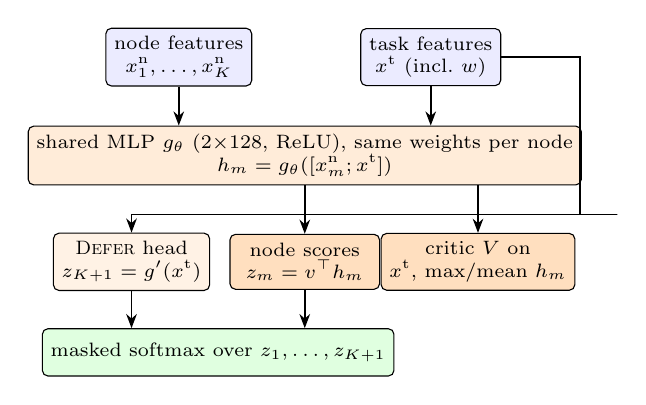
\begin{tikzpicture}[node distance=0.32cm]
\node[blk,fill=blue!8] (xn) at (0,0) {node features\\$x^{\mathrm n}_1,\dots,x^{\mathrm n}_K$};
\node[blk,fill=blue!8] (xt) at (3.2,0) {task features\\$x^{\mathrm t}$ (incl.\ $w$)};
\node[blk,fill=orange!15,minimum width=6.4cm] (mlp) at (1.6,-1.25) {shared MLP $g_\theta$ (2$\times$128, ReLU), same weights per node\\$h_m=g_\theta([x^{\mathrm n}_m;x^{\mathrm t}])$};
\node[blk,fill=orange!10,minimum width=1.9cm] (df) at (-0.6,-2.6) {\textsc{Defer} head\\$z_{K+1}=g'(x^{\mathrm t})$};
\node[blk,fill=orange!25,minimum width=1.9cm] (sc) at (1.6,-2.6) {node scores\\$z_m=v^\top h_m$};
\node[blk,fill=orange!25,minimum width=1.9cm] (cr) at (3.8,-2.6) {critic $V$ on\\$x^{\mathrm t}$, max/mean $h_m$};
\node[blk,fill=green!12] (sm) at (0.5,-3.75) {masked softmax over $z_1,\dots,z_{K+1}$};
\draw[arr] (xn)--(xn|-mlp.north); \draw[arr] (xt)--(xt|-mlp.north);
\draw[arr] (mlp.south-|sc)--(sc); \draw[arr] (mlp.south-|cr)--(cr);
\draw[arr] (xt.east) -- ++(1.0,0) |- ($(mlp.east)+(0.45,-0.75)$) -| (df.north);
\draw[arr] (df.south)--(df.south|-sm.north); \draw[arr] (sc.south)--(sc.south|-sm.north);
\end{tikzpicture}
\caption{Policy and critic. The scorer is shared across nodes, so the network ($\approx$60\,K parameters) works for any number of nodes and a failed node is simply masked.}
\label{fig:net}
\end{figure}

The policy (Fig.~\ref{fig:net}) applies one MLP $g_\theta$ to every node's features concatenated with the task features, giving $h_m=g_\theta([x^{\mathrm n}_m;x^{\mathrm t}])$ and a score $z_m=v^\top h_m$; a small head scores \textsc{Defer} from $x^{\mathrm t}$. With the action mask $\mathcal M$,
\begin{equation}
\pi_\theta(a\mid s,w) = \frac{\exp(z_a)\,\mathbb 1[a\in\mathcal M]}{\sum_{a'\in\mathcal M}\exp(z_{a'})}. \label{eq:policy}
\end{equation}
The critic reads $x^{\mathrm t}$ and the max- and mean-pooled $h_m$. Inference takes about 0.55\,ms on one CPU core.

\subsection{Training}
\textbf{Behaviour cloning.} Three iterations minimise the cross-entropy to the actions of the carbon-aware heuristic CA-EFT (Section~\ref{sec:setup}), $\mathcal L_{\mathrm{BC}} = -\mathbb E\left[\ln\pi_\theta(a^{\mathrm{CA}}\mid s,w)\right]$.

\textbf{Preference-conditioned PPO.} Each episode samples $w\sim U[0,1]$, so one network learns the whole trade-off. With advantages $\hat A_k$ from generalised advantage estimation ($\lambda=0.9$) and $\rho_k(\theta)=\pi_\theta(a_k\mid s_k,w)/\pi_{\theta_{\mathrm{old}}}(a_k\mid s_k,w)$, we minimise
\begin{multline}
\mathcal L(\theta) = -\mathbb E_k\!\left[\min\!\big(\rho_k\hat A_k,\ \mathrm{clip}(\rho_k,0.8,1.2)\hat A_k\big)\right] \\
+ 0.5\,\mathbb E_k\!\left[(V_\theta(s_k)-\hat R_k)^2\right] - \beta\,\mathbb E_k\!\left[\mathcal H(\pi_\theta(\cdot\mid s_k))\right], \label{eq:ppo}
\end{multline}
with learning rate $3\cdot10^{-4}$, four epochs per iteration, gradient-norm clipping at 0.5, and the entropy weight $\beta$ decaying from 0.01 to 0.002.

\textbf{Domain randomisation.} Every episode draws 2--6 edge, 1--3 fog and 1--3 cloud nodes, server speeds $\pm$20\%, RTT $\times$0.7--1.5, bandwidth $\times$0.5--1.5, alert rate 0.1--0.4 per camera per second, analytics load proportional to the server count and estimate noise $\sigma\in[0,0.4]$. The final model trained for 82 PPO iterations (about 3.5\,M decisions, 35 minutes on a laptop CPU); Fig.~\ref{fig:train} shows the curves. Algorithm~\ref{alg:train} summarises training.

\begin{algorithm}[t]
\caption{PACE training}
\label{alg:train}
\begin{algorithmic}[1]
\REQUIRE dataset train split, CA-EFT teacher, iterations $N$
\STATE $\theta\leftarrow$ random; collect CA-EFT decisions in randomised simulators
\FOR{3 iterations}
  \STATE minimise $\mathcal L_{\mathrm{BC}}$ on the teacher's actions
\ENDFOR
\FOR{$it=1$ \TO $N$}
  \FOR{each parallel worker}
    \STATE sample topology, load, network, noise; sample $w\sim U[0,1]$
    \STATE run $\pi_\theta$ for 6000 decisions; compute $r_i$ by \eqref{eq:reward} when jobs finish
  \ENDFOR
  \STATE compute $\hat A_k$ with GAE; 4 epochs of minibatch updates on \eqref{eq:ppo}
\ENDFOR
\STATE (testbed) calibrate twin; fine-tune $\theta$ in the twin; select on train-split validation
\end{algorithmic}
\end{algorithm}

\begin{figure}[t]
\centering
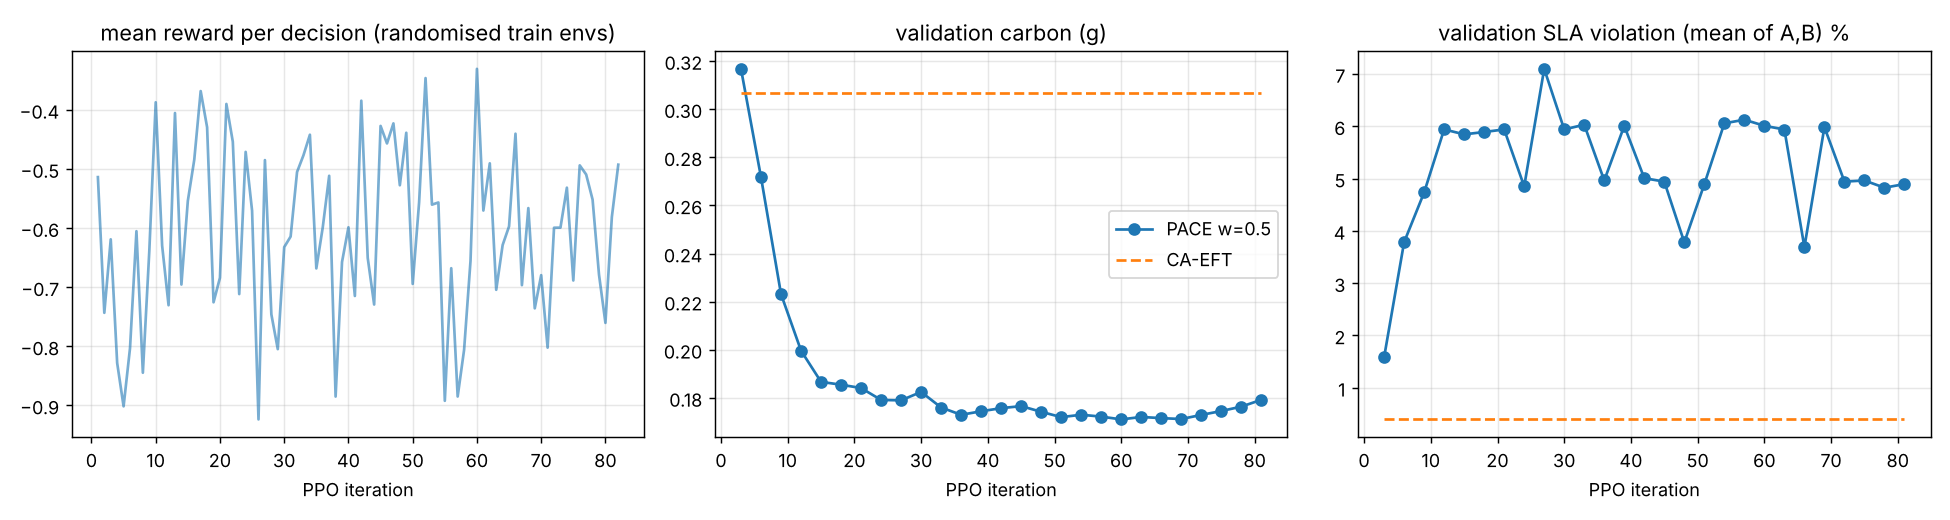
\includegraphics[width=\columnwidth]{training.png}
\caption{Training: mean reward per decision (left), and validation carbon and SLA violations against CA-EFT.}
\label{fig:train}
\end{figure}

\subsection{SLA-target controller and safety shield}\label{sec:ctrl}
Because $w$ is an input, changing it changes behaviour instantly. After every ten completed class A/B jobs, with $\bar m$ the miss rate of the last 50 and target $\varepsilon$,
\begin{equation}
e=\bar m-\varepsilon,\quad I\leftarrow\mathrm{clip}(I+e,-5,5),\quad w=\mathrm{clip}(w_0+K_pe+K_iI,0,1), \label{eq:pi}
\end{equation}
with $K_p=0.8$ and $K_i=0.08$. This is the deployment-time analogue of a Lagrange multiplier on $\mathrm{SLA}\le\varepsilon$~\cite{stooke2020}. A new target resets $I$ (anti-windup).

The shield keeps only nodes with
\begin{equation}
\hat f_{in}-t \le (1-0.6\,w)\,b_i, \label{eq:shield}
\end{equation}
i.e.\ 40\% of the budget at $w=1$ and the full budget at $w=0$; if no node qualifies it abstains. Algorithm~\ref{alg:online} shows the online loop.

\begin{algorithm}[t]
\caption{PACE online scheduling}
\label{alg:online}
\begin{algorithmic}[1]
\REQUIRE policy $\pi_\theta$, target $\varepsilon$, initial $w_0$
\LOOP
  \STATE wait for an event (task ready, wake-up, failure, completion)
  \IF{completion of a class A/B job}
    \STATE update $\bar m$; every 10 jobs update $w$ by \eqref{eq:pi}
  \ENDIF
  \FOR{each ready task $i$ (time frozen)}
    \STATE build $x^{\mathrm t}$, $x^{\mathrm n}_m$ using \eqref{eq:finish} plus the online network estimate
    \STATE mask infeasible actions; apply shield \eqref{eq:shield}
    \STATE $a\leftarrow\arg\max_a\pi_\theta(a\mid s,w)$; place $i$ on $a$ or defer it
  \ENDFOR
\ENDLOOP
\end{algorithmic}
\end{algorithm}

% ==================================================================== V
\section{Experimental Setup}\label{sec:setup}
\textbf{Simulator.} A discrete-event simulator implements \eqref{eq:transfer}--\eqref{eq:carbon} with log-normal transfer jitter, failures and stragglers; schedulers see only estimates. Topologies: \emph{testbed} (2 edge, 2 fog, 2 cloud) and \emph{city} (8 edge, 3 fog, 4 cloud). Carbon traces are synthetic hourly profiles built from real annual means (IN-SO 560, IN-WE 680, SE-SE3 35\,\gco/kWh) with a solar dip, an evening peak and autocorrelated noise.

\textbf{Baselines.} Random; edge-, fog- and cloud-only; carbon-greedy; EFT (earliest estimated finish); Job-EFT; MERSEM with $w_s\in\{1,0.5,0\}$ and an oracle variant; and CA-EFT, the strongest hand-made rule:
\begin{equation}
a^{\mathrm{CA}} = \begin{cases}\arg\min_{n\in S} \hat C_{in}, & S=\{n:\hat f_{in}-t\le\mu b_i\}\neq\emptyset\\ \arg\min_n \hat f_{in}, & \text{otherwise,}\end{cases}
\end{equation}
with margin $\mu=0.4$ tuned on training seeds.

\textbf{MERSEM re-implementation.} We follow the paper where it is specific (job-level placement, epoch planning, objective \eqref{eq:mersem}, dominance-based replacement, Q-learning-guided local search on 30\% of the population with $\alpha=0.15$, $\gamma=0.9$, five actions) and document the rest (population 20, 30 generations per epoch, uniform crossover). We are generous: its predictor sees the \emph{actual} next-epoch arrivals, its population is seeded with an EFT mapping and unplanned or failed placements fall back to EFT.

\textbf{Protocol.} All methods see the same jobs and carbon trace per seed (held-out jobs only); 10 seeds for E1 and E6, 5 for stress tests. We report means, paired Wilcoxon signed-rank tests, and the Pareto hypervolume $\mathrm{HV}=\lambda\big(\bigcup_{p\in P}[p,r]\big)$ of each method's front $P$ in (SLA, carbon) with reference point $r$ at 1.05$\times$ the worst point. PACE uses $w=0.9$ unless stated.

% ==================================================================== VI
\section{Simulation Results}\label{sec:sim}

\begin{table}[t]
\caption{E1: testbed topology, nominal load, 10 paired seeds}
\label{tab:e1}
\centering\scriptsize
\setlength{\tabcolsep}{3pt}
\begin{tabular}{@{}lrrrrr@{}}
\toprule
Method & A miss & B miss & A+B miss & Carbon (g) & p95 A (s)\\
\midrule
EFT & 10.4\% & 1.3\% & 10.3\% & 1.96 & 1.29\\
Carbon-greedy & 65.8\% & 77.0\% & 66.0\% & 0.28 & 5.11\\
CA-EFT & 2.8\% & 5.6\% & 2.8\% & 0.74 & 0.80\\
MERSEM-SLA & 6.7\% & 33.6\% & 7.1\% & 1.82 & 1.31\\
MERSEM-Balanced & 12.7\% & 45.4\% & 13.3\% & 0.51 & 2.20\\
MERSEM-Bal.\ oracle & 10.7\% & 45.3\% & 11.3\% & 0.49 & 2.25\\
\midrule
\textbf{PACE} ($w$=0.9) & \textbf{0.9\%} & 23.1\% & \textbf{1.3\%} & \textbf{0.39} & 0.84\\
\textbf{PACE+shield} ($w$=1) & 1.8\% & 6.0\% & 1.9\% & 0.55 & 0.87\\
PACE+shield, $\varepsilon$=2\% & 1.8\% & 16.2\% & 2.1\% & 0.47 & 0.83\\
\bottomrule
\end{tabular}
\end{table}

\subsection{Nominal load (E1)}
Table~\ref{tab:e1}: against MERSEM-Balanced, PACE misses 12\pp\ fewer deadlines with 22\% less dynamic carbon, better in every seed ($p=0.002$). Against CA-EFT it misses 1.5\pp\ fewer with 47\% less carbon ($p=0.01$, $0.002$). On the city topology the gap to MERSEM is 17\pp\ (1.0\% vs 17.9\%) and 34\% carbon. The one-policy front has the largest hypervolume (Fig.~\ref{fig:pareto}): PACE 1172, PACE+shield 1156, CA-EFT 1131, MERSEM 1083 (city: 2626, 2612, 2565, 2287).

The weakness is analytics: pure PACE misses 23\% of class-B jobs against CA-EFT's 5.6\%. Alerts are 98\% of jobs, the held-out DAGs are larger (median 25 vs 15 tasks), and \eqref{eq:reward} does not charge a placement for the delay it causes other jobs, so the policy overloads the small green cloud. The shield closes most of the gap (6.0\%).

\begin{figure}[t]
\centering
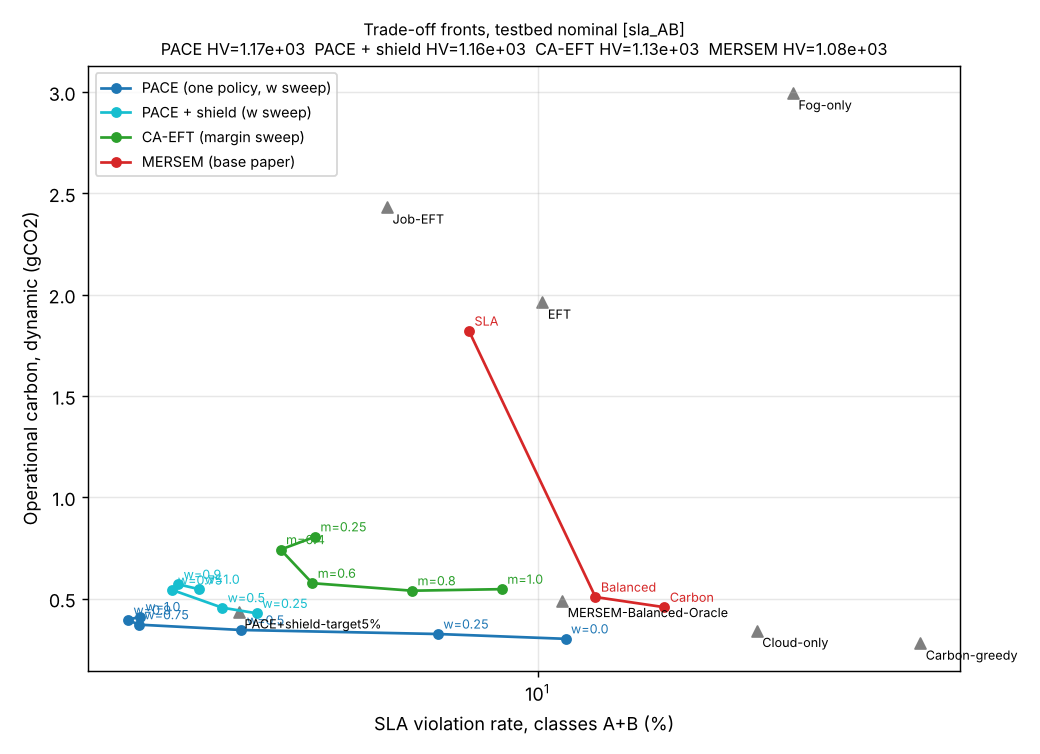
\includegraphics[width=\columnwidth]{pareto_testbed.png}
\caption{SLA--carbon fronts on the testbed topology: one PACE policy sweeping $w$, CA-EFT sweeping its margin, MERSEM its three weights.}
\label{fig:pareto}
\end{figure}

\subsection{Stress tests (E2--E5)}
\begin{table}[t]
\caption{A+B misses under stress, 5 paired seeds}
\label{tab:stress}
\centering\scriptsize
\setlength{\tabcolsep}{3pt}
\begin{tabular}{@{}lrrrr@{}}
\toprule
Scenario & MERSEM & CA-EFT & PACE & PACE+sh.\\
\midrule
1.5$\times$ load & 22.8\% & 4.5\% & \textbf{1.9\%} & 2.5\%\\
2$\times$ load & 26.3\% & 7.2\% & \textbf{3.0\%} & 4.8\%\\
Estimate noise $\sigma$=0.4 & 14.0\% & 3.2\% & \textbf{1.2\%} & 1.4\%\\
Fog crash + stragglers & 26.4\% & 15.9\% & 14.8\% & \textbf{11.0\%}\\
Random failures & 18.6\% & 4.0\% & \textbf{1.8\%} & 2.7\%\\
Rush hour ($\times$2.5, 15 min)$^{\mathrm a}$ & 22.0\% & 4.9\% & -- & \textbf{2.8\%}\\
\bottomrule
\multicolumn{5}{@{}l}{$^{\mathrm a}$PACE+shield at $w$=0.5.}
\end{tabular}
\end{table}

A PACE variant has the fewest violations in every scenario (Table~\ref{tab:stress}), and PACE uses less carbon than CA-EFT in each. PACE decides when each task is ready, so a crashed node is masked and its tasks re-placed, while MERSEM's epoch plan goes stale (Fig.~\ref{fig:rush}).

\begin{figure}[t]
\centering
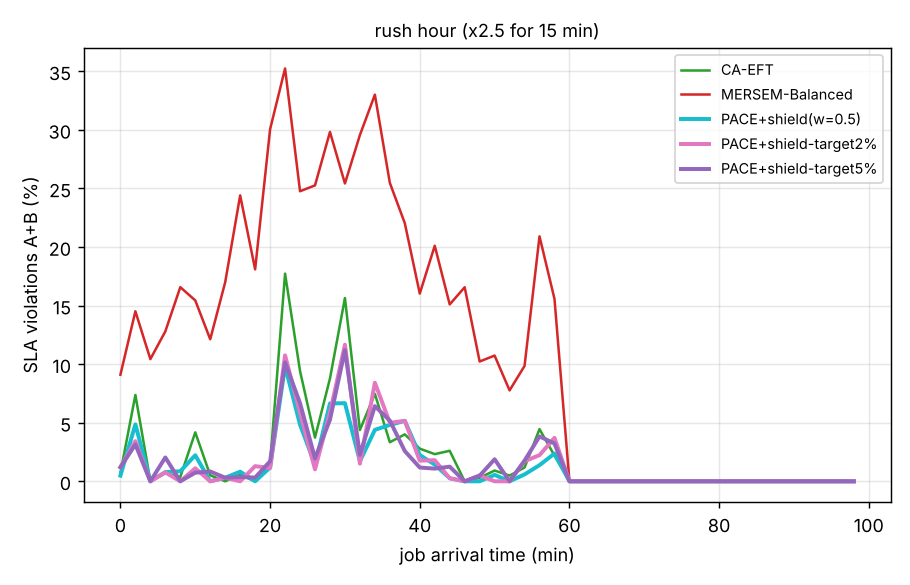
\includegraphics[width=\columnwidth]{e5_rush_hour.png}
\caption{Misses over a one-hour run with a 15-minute rush hour from minute 20.}
\label{fig:rush}
\end{figure}

\subsection{Holding an SLA target}
With $\varepsilon=2\%$ the controller achieved 2.0\% on the testbed topology and 1.7\% on the city; the daily $w$ settled between 0.25 and 0.87, adapting to load and grid. A loose 5\% target gave 2.3\% misses and spent the headroom on carbon ($-25\%$ vs fixed $w=0.9$). A fixed-weight method must re-run its search to reach a target.

\subsection{Generalisation to unseen setups (E6)}
Without retraining, we tested setups outside the training ranges (Table~\ref{tab:e6}). The larger city exceeded the implementation's buffer of 12 candidate nodes; because the scorer is shared, we only let the buffer grow (identical results for $\le$12 nodes). On the first four setups PACE beat both baselines in 10/10 seeds ($p=0.002$) with less carbon (e.g.\ $-38\%$ vs MERSEM, $-44\%$ vs CA-EFT on the larger city). It \emph{fails} on a much slower WAN: it keeps sending alerts to Stockholm, while CA-EFT recomputes finish times. The real testbed showed the same weakness (Section~\ref{sec:real}).

\begin{table}[t]
\caption{E6: A+B misses on unseen setups, 10 paired seeds}
\label{tab:e6}
\centering\scriptsize
\setlength{\tabcolsep}{3pt}
\begin{tabular}{@{}lrrr@{}}
\toprule
Setup & PACE & CA-EFT & MERSEM\\
\midrule
Seen: city 8/3/4 nodes & \textbf{1.0\%} & 2.8\% & 17.9\%\\
2$\times$ larger city (16/6/8) & \textbf{0.4\%} & 4.6\% & 17.3\%\\
Cloud in Frankfurt (unseen zone) & \textbf{0.7\%} & 2.8\% & 16.2\%\\
2$\times$ work, 3$\times$ data & \textbf{2.7\%} & 7.6\% & 27.8\%\\
Slow WAN (RTT$\times$2, BW$\times$0.3) & 17.3\% & \textbf{1.4\%} & 24.8\%\\
\bottomrule
\end{tabular}
\end{table}

% ==================================================================== VII
\section{Real AWS Testbed}\label{sec:real}

\begin{figure}[t]
\centering
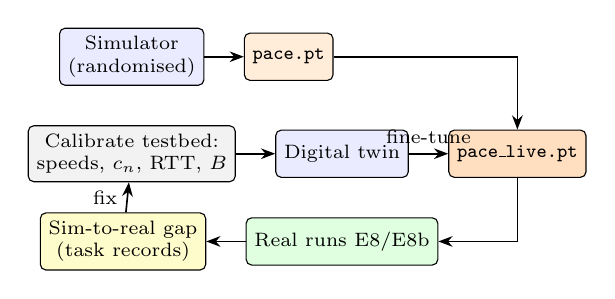
\begin{tikzpicture}[node distance=0.32cm]
\node[blk,fill=blue!8] (sim) {Simulator\\(randomised)};
\node[blk,fill=orange!15,right=0.5cm of sim] (pt) {\texttt{pace.pt}};
\node[blk,fill=gray!10,below=0.5cm of sim] (cal) {Calibrate testbed:\\speeds, $c_n$, RTT, $B$};
\node[blk,fill=blue!8,right=0.5cm of cal] (twin) {Digital twin};
\node[blk,fill=orange!25,right=0.5cm of twin] (live) {\texttt{pace\_live.pt}};
\node[blk,fill=green!12,below=0.5cm of twin] (run) {Real runs E8/E8b};
\node[blk,fill=yellow!20,left=0.5cm of run] (gap) {Sim-to-real gap\\(task records)};
\draw[arr] (sim)--(pt); \draw[arr] (cal)--(twin); \draw[arr] (pt) -| (live); \draw[arr] (twin)--node[above,font=\scriptsize]{fine-tune}(live);
\draw[arr] (live) |- (run); \draw[arr] (run)--(gap); \draw[arr] (gap)--node[left,font=\scriptsize]{fix}(cal);
\end{tikzpicture}
\caption{Sim-to-real loop: calibrate, fine-tune in the twin, run for real, find the gap in the task records, fix the model.}
\label{fig:loop}
\end{figure}

\subsection{Setup}
Two laptop processes act as one-core camera boxes in Coimbatore (3$\times$ slower than a cloud vCPU). The fog and cloud each have an x86 \texttt{c7i-flex.large} and an ARM \texttt{t4g.small} instance. Workers run real tasks: a BLAS kernel for analytics and OpenCV HOG pedestrian detection for camera frames. The laptop orchestrator runs the same scheduler code as the simulator and a live dashboard with failure, carbon-spike, rush-hour and SLA-target controls. Runs last 6 minutes and the schedulers are interleaved per seed so they share network conditions.

\subsection{Calibration and three sim-to-real gaps}
Following the loop in Fig.~\ref{fig:loop}, a calibration script measures node speeds per task type, $c_n$, RTT and bandwidth; the simulator so configured is a digital twin used to predict every experiment beforehand. Three gaps emerged. (1) \emph{Dispatch}: the orchestrator held a slot during a task's whole HTTP round trip and the twin had no controller round trip; tasks are now dispatched at placement, inputs fetched while others compute, and every scheduler sees the round trip. (2) \emph{SMT contention}: a 2-vCPU x86 instance is one physical core, so two concurrent tasks each ran 1.7--1.8$\times$ slower (assumed 1.15); calibration now measures $c_n$ per node. (3) \emph{Network drift}: in the first real run (E8) the median network time of alert detections to Mumbai grew from 0.25\,s to about 0.5\,s over the evening, and PACE (14.7\% missed) lost to MERSEM (10.3\%), which ran more detections on the edge. We added an online estimate: for region $r$, with residuals $\delta=T^{\mathrm{net}}_{\mathrm{measured}}-T^{\mathrm{net}}_{\mathrm{model}}$ of the last 30 tasks,
\begin{equation}
\hat T^{\mathrm{net}}_{r} \leftarrow T^{\mathrm{net}}_{\mathrm{model},r} + q_{0.9}\big(\{\delta\}_{\mathrm{last}\,30}\big), \label{eq:online}
\end{equation}
used by every scheduler, by PACE's features and by the shield. PACE was fine-tuned in three stages as the twin was corrected.

\subsection{Results with the online estimate (E8b)}
\begin{table}[t]
\caption{Real testbed, E8b, 3 seeds per load (A+B misses, dynamic carbon per run)}
\label{tab:e8b}
\centering\scriptsize
\setlength{\tabcolsep}{3pt}
\begin{tabular}{@{}lrrrr@{}}
\toprule
& \multicolumn{2}{c}{Nominal} & \multicolumn{2}{c}{Busy hour}\\
\cmidrule(lr){2-3}\cmidrule(l){4-5}
Scheduler & Miss & g & Miss & g\\
\midrule
MERSEM-Balanced & 9.4\% & 0.037 & 14.3\% & 0.063\\
CA-EFT & 3.7\% & 0.051 & 6.2\% & 0.083\\
EFT & 14.4\% & 0.282 & -- & --\\
\textbf{PACE} & 3.8\% & 0.044 & 6.6\% & 0.067\\
\textbf{PACE+shield} & 6.1\% & 0.050 & \textbf{4.6\%}$^{\mathrm a}$ & 0.069\\
\bottomrule
\multicolumn{5}{@{}l}{$^{\mathrm a}$No alert deadline missed.}
\end{tabular}
\end{table}

\begin{table}[t]
\caption{Paired comparison over the six E8b runs (Wilcoxon; min.\ attainable $p$=0.031)}
\label{tab:paired}
\centering\scriptsize
\setlength{\tabcolsep}{2.5pt}
\begin{tabular}{@{}llrrrrr@{}}
\toprule
Variant & vs & Better & $\Delta$miss & $p$ & $\Delta$CO$_2$ & $p$\\
\midrule
PACE & MERSEM & 6/6 & $-6.6$\pp & 0.031 & +15\% & 0.156\\
PACE & CA-EFT & 2/6 & $+0.2$\pp & 0.875 & $-15\%$ & 0.031\\
PACE+sh. & MERSEM & 4/6 & $-6.4$\pp & 0.156 & +25\% & 0.094\\
PACE+sh. & CA-EFT & 4/6 & $+0.4$\pp & 1.000 & $-9\%$ & 0.156\\
\bottomrule
\end{tabular}
\end{table}

PACE missed fewer deadlines than MERSEM in all six paired runs (Tables~\ref{tab:e8b} and~\ref{tab:paired}), in alerts and analytics, for 15\% more carbon on average (not significant): at $w=0.9$ PACE favours deadlines while MERSEM-Balanced sits at a lower-carbon, higher-miss point. Against CA-EFT it had the same deadline performance with 15\% less carbon. EFT used about 6$\times$ PACE's carbon (Fig.~\ref{fig:real}).

\begin{figure}[t]
\centering
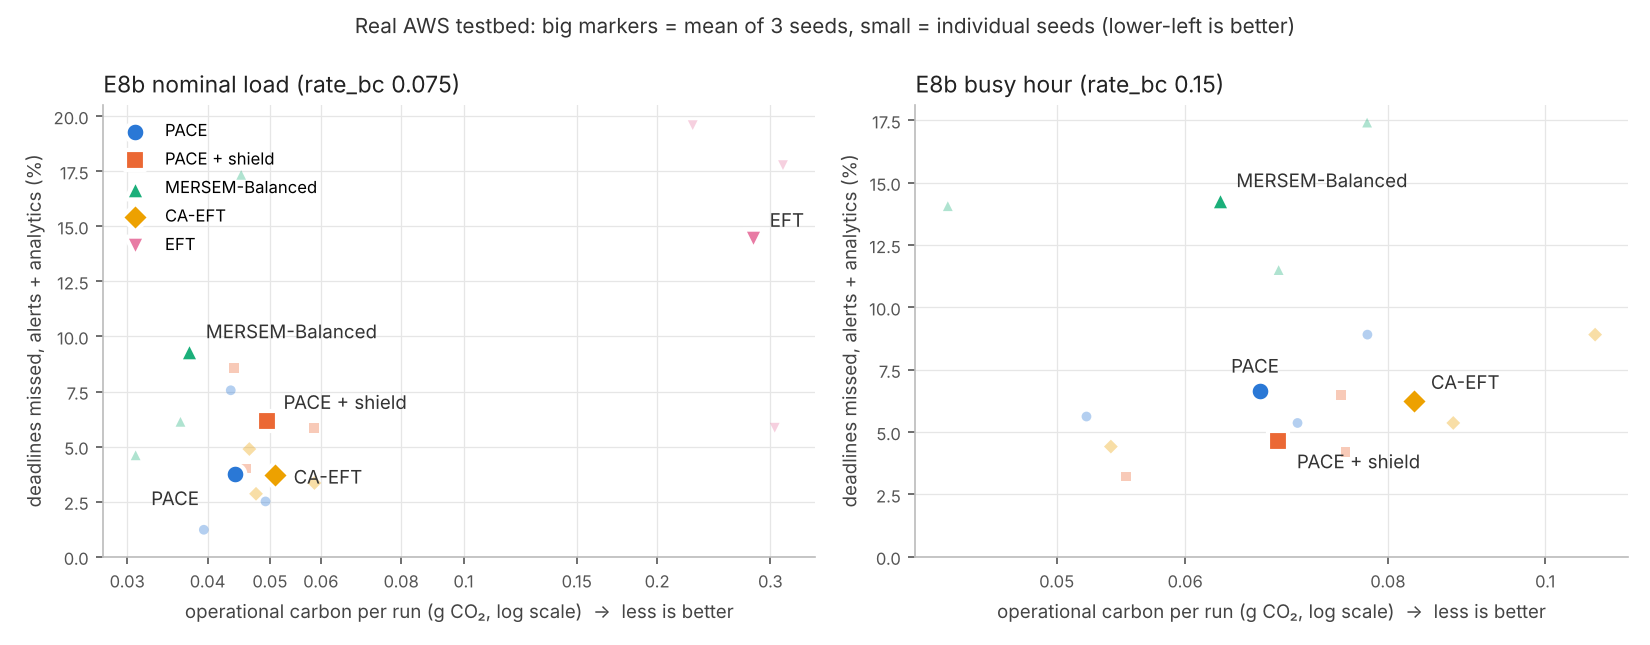
\includegraphics[width=\columnwidth]{e8_real.png}
\caption{Real testbed (E8b): misses against dynamic carbon, nominal load and busy hour.}
\label{fig:real}
\end{figure}

\subsection{Sim-to-real fidelity and live demonstration}
Replaying each real job trace in the twin (E9) shows it is optimistic, mostly about alert latency (e.g.\ PACE+shield, busy hour: 6.5/4.2/3.2\% real vs 6.5/3.8/2.4\% predicted; larger gaps at nominal load), because the campus uplink varies more than the twin's static link model (Fig.~\ref{fig:e9}). In a rehearsed live demonstration with a street video as the camera feed, a four-fold carbon spike kept work off Mumbai, a three-fold rush hour missed 0.7\% of alerts (p95 0.45\,s), a crashed Mumbai node was masked for 60\,s with its tasks re-placed, and moving $\varepsilon$ from 5\% to 1\% raised $w$ from 0.77 to 0.89 within 30\,s without retraining.

\begin{figure}[t]
\centering
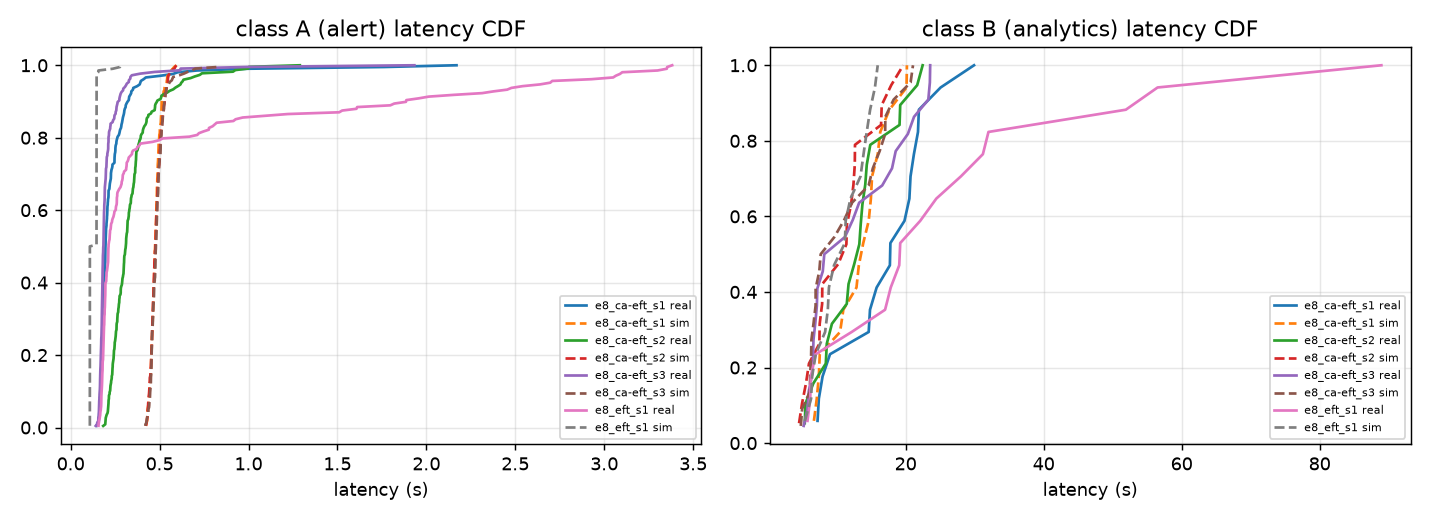
\includegraphics[width=\columnwidth]{e9_latency_cdf.png}
\caption{E9: real versus simulated latency distributions on identical job traces.}
\label{fig:e9}
\end{figure}

% ==================================================================== VIII
\section{Discussion and Limitations}
PACE is strongest for tight-deadline alerts, under load, failures and estimate errors, on larger or different topologies including an unseen grid zone, and when the objective must change at run time. It is weaker on large analytics DAGs without the shield (23\% vs 6\% in simulation), on networks far outside training (17\% vs 1.4\% on the slow WAN, and E8 before the online estimate), and on the real testbed MERSEM used about 15\% less carbon at many more misses.

\textbf{Threats to validity.} Carbon intensities are synthetic profiles from real annual means: free hourly data for the Indian zones was unavailable to us (the code reads Electricity Maps CSVs). The India--Sweden gap drives most decisions, so we expect the ranking to hold, but this is untested. Energy is modelled from CPU time and published coefficients because AWS exposes no per-VM power. The testbed is small (six nodes, three seeds per load, one campus network), and MERSEM is a re-implementation, to which we were deliberately generous.

% ==================================================================== IX
\section{Conclusion}
PACE turns edge--cloud scheduling into an online, task-level decision taken in about a millisecond by one preference-conditioned policy. In simulation it misses an order of magnitude fewer deadlines than MERSEM with less carbon, keeps its lead under stress and on most unseen setups, and lets operators set an SLA target at run time. On a real three-region testbed it missed fewer deadlines than MERSEM in every paired run and matched the best heuristic with 15\% less carbon; building the testbed exposed three sim-to-real gaps that simulation alone would have hidden. Future work: a graph neural network encoder over the job DAG, wider network randomisation with the online estimate inside training, PPO-Lagrangian as an alternative to the PI controller, real hourly carbon traces, and a longer testbed campaign. Code and data: \url{https://github.com/p-art-dheev/RL-Project}.

\section*{Acknowledgment}
We thank our guide, Dr.\ Palmani Duraisamy, for guidance throughout this project.

% ==================================================================== references
\begin{thebibliography}{00}
\bibitem{mersem} P. Ramicetty \emph{et al.}, ``Sustainable graph analytics workload scheduling with evolutionary reinforcement learning in edge-cloud systems,'' arXiv:2605.13489, 2026.
\bibitem{dataset} S. A. Ali Rezaee and S. Adabi, ``Jobs (DAG workflow) and tasks dataset,'' Zenodo, doi:10.5281/zenodo.4667690.
\bibitem{edgecloudsim} C. Sonmez, A. Ozgovde, and C. Ersoy, ``EdgeCloudSim: An environment for performance evaluation of edge computing systems,'' in \emph{Proc. FMEC}, 2017.
\bibitem{deeprm} H. Mao, M. Alizadeh, I. Menache, and S. Kandula, ``Resource management with deep reinforcement learning,'' in \emph{Proc. ACM HotNets}, 2016.
\bibitem{deeprm2} Y. Ye \emph{et al.}, ``A new approach for resource scheduling with deep reinforcement learning,'' arXiv:1806.08122, 2018.
\bibitem{decima} H. Mao \emph{et al.}, ``Learning scheduling algorithms for data processing clusters,'' in \emph{Proc. ACM SIGCOMM}, 2019.
\bibitem{wang2021} J. Wang \emph{et al.}, ``Dependent task offloading for edge computing based on deep reinforcement learning,'' \emph{IEEE Trans. Comput.}, 2021.
\bibitem{abels2019} A. Abels \emph{et al.}, ``Dynamic weights in multi-objective deep reinforcement learning,'' in \emph{Proc. ICML}, 2019.
\bibitem{yang2019} R. Yang, X. Sun, and K. Narasimhan, ``A generalized algorithm for multi-objective reinforcement learning and policy adaptation,'' in \emph{Proc. NeurIPS}, 2019.
\bibitem{stooke2020} A. Stooke, J. Achiam, and P. Abbeel, ``Responsive safety in reinforcement learning by PID Lagrangian methods,'' in \emph{Proc. ICML}, 2020.
\bibitem{ray2019} A. Ray, J. Achiam, and D. Amodei, ``Benchmarking safe exploration in deep reinforcement learning,'' OpenAI, 2019.
\bibitem{wiesner2021} P. Wiesner \emph{et al.}, ``Let's wait awhile: How temporal workload shifting can reduce carbon emissions in the cloud,'' in \emph{Proc. ACM/IFIP Middleware}, 2021.
\bibitem{ppo} J. Schulman \emph{et al.}, ``Proximal policy optimization algorithms,'' arXiv:1707.06347, 2017.
\bibitem{ccf} Cloud Carbon Footprint, ``Methodology,'' [Online]. Available: https://www.cloudcarbonfootprint.org/docs/methodology
\end{thebibliography}

\end{document}
